\section{Instruction Set Architecture}

All computers share similar constraints in designing instructions.
The specifications for a machine's instructions and functional
operation are called an \emph{instruction set architecture} (ISA).
The fundamentals of one flavor of ISA extrapolate to another.
In this class, we study the fundamental subset of RISC-V that is common to all ISAs.

\subsection{Register Arithmetic}

Recall the example of converting C to assembly.
\begin{lstlisting}
    f = (g + h) - (i + j);
    // add t0, g, h
    // add t1, i, j
    // sub f, t0, t1
\end{lstlisting}

\texttt{g}, \texttt{h}, \texttt{i}, \texttt{j}, \texttt{t0},
and \texttt{t1} are the operands and are stored in \emph{registers}.
Registers are word-sized (typically, 8- to 64-bit) storage
elements inside the core itself.
\marginnote{
    The RISC-V 32I ISA has 32-bit registers: \texttt{x0}-\texttt{x31}.
}
The 32 registers in 32-bit architecture
are fast locations for storing and
accessing data. In RISC-V, data must be
in registers to perform arithmetic. Register
\texttt{x0} always equals zero.
In addition to the registers, there
are also $2^{30}$ memory words accessed
only by data transfer instructions.
RISC-V uses byte addresses, so sequential
word accesses differ by 4. Memory holds
data structures, arrays, and spilled
registers.

The RISC-V assembly language has
instructions like in Table \ref{tab:riscvasmarithmetic}.
\begin{table}[h!]
    \begin{tabular}{lll}
        Instruction                   & Example                  & Meaning               \\
        Add                           & \texttt{add x5, x6, x7}  & \texttt{x5 = x6 + x7} \\
        Subtract                      & \texttt{sub x5, x6, x7}  & \texttt{x5 = x6 - x7} \\
        Add immediate (for constants) & \texttt{addi x5, x6, 20} & \texttt{x5 = x6 + 20}
    \end{tabular}
    \caption{RISC-V Assembly Arithmetic}
    \label{tab:riscvasmarithmetic}
\end{table}

\begin{lstlisting}[]
    main:
        li x10, 1 // li = load immediate
        li x11, 2 // manually initialize
        li x12, 4
        li x13, 5

        add x10, x10, x11 // now, x10 = x10 + x11
        add x12, x12, x13 // now, x12 = x12 + x13
        add x10, x10, x12 // now, x10 = (x10 + x11) + (x12 + x13)
\end{lstlisting}

There are general purpose and special
registers, as tabulated in Table \ref{tab:registers}.
\begin{table}[h!]
    \centering
    \begin{tabular}{|c|c|c|c|}
        \hline
        \textbf{Register} & \textbf{ABI Name} & \textbf{Description}             & \textbf{Saver} \\
        \hline
        x0                & zero              & Hardwired zero                   & -              \\
        x1                & ra                & Return address                   & Caller         \\
        x2                & sp                & Stack pointer                    & Callee         \\
        x3                & gp                & Global pointer                   & -              \\
        x4                & tp                & Thread pointer                   & -              \\
        x5                & t0                & Temporary register               & Caller         \\
        x6                & t1                & Temporary register               & Caller         \\
        x7                & t2                & Temporary register               & Caller         \\
        x8                & s0/fp             & Saved register / Frame pointer   & Callee         \\
        x9                & s1                & Saved register                   & Callee         \\
        x10               & a0                & Function argument / Return value & Caller         \\
        x11               & a1                & Function argument / Return value & Caller         \\
        x12               & a2                & Function argument                & Caller         \\
        x13               & a3                & Function argument                & Caller         \\
        x14               & a4                & Function argument                & Caller         \\
        x15               & a5                & Function argument                & Caller         \\
        x16               & a6                & Function argument                & Caller         \\
        x17               & a7                & Function argument                & Caller         \\
        x18               & s2                & Saved register                   & Callee         \\
        x19               & s3                & Saved register                   & Callee         \\
        x20               & s4                & Saved register                   & Callee         \\
        x21               & s5                & Saved register                   & Callee         \\
        x22               & s6                & Saved register                   & Callee         \\
        x23               & s7                & Saved register                   & Callee         \\
        x24               & s8                & Saved register                   & Callee         \\
        x25               & s9                & Saved register                   & Callee         \\
        x26               & s10               & Saved register                   & Callee         \\
        x27               & s11               & Saved register                   & Callee         \\
        x28               & t3                & Temporary register               & Caller         \\
        x29               & t4                & Temporary register               & Caller         \\
        x30               & t5                & Temporary register               & Caller         \\
        x31               & t6                & Temporary register               & Caller         \\
        \hline
    \end{tabular}
    \caption{RISC-V Registers}
    \label{tab:registers}
\end{table}

The operands for arithmetic instructions
always come from registers. If the
values of an operand is known ahead
of time, then \texttt{addi} can be used.
This is useful for adding constants to
operands.

An \emph{addressing mode} defines how an operand gets its
values. All ISAs have a limited number of registers.
The more you add, the slower they get and the more
circuitry required to access. That means virtually all
machines have memory, which is byte-addresses. Address
0 is byte 0, address 1 is byte 1, etc. An ISA defines
many things, including the interaction between processor
and memory. For instance, two different ISAs
may compute "Z = X + Y" differently. One might
use the accumulator method consisting of
\begin{lstlisting}
    LoadA X
    AddA Y
    StoreA Z
\end{lstlisting}
while most others use the reg/reg method of
\begin{lstlisting}
    Load R1, X
    Load R2, Y
    Add  R3, R1, R2
    Store R3, Z
\end{lstlisting}

Basic memory instructions in RISC-V are
\begin{table}{h!}
    \begin{tabular}{llll}
        Load word           & \texttt{lw x5, 40(x6)}  & \texttt{x5 = Memory[x6 + 40]} & Word from memory to register          \\
        Load word, unsigned & \texttt{lwu x5, 40(x6)} & \texttt{x5 = Memory[x6 + 40]} & Unsigned word from memory to register \\
        Store word          & \texttt{sw x5, 40(x6)}  & \texttt{Memory[x6 + 40] = x5} & Word from register to memory
    \end{tabular}
\end{table}

Memory in RISC-V is byte-addressed.
4B, 2B, and 1B memory operations are
all available. All registers on the
RISC-V machine are 32 bits (4B).
When you load something less than 4 bytes,
the upper bits are generally zeroed or
sign extended.

An addressing mode defines how an operand gets its values.
\begin{itemize}
    \item Register addressing: read the value from a register
    \item Immediate addressing: read the value from a constant
          burned into the instruction.
    \item Offset addressing: read the value from memory.
          The address is computed by adding an immediate to the value
          in the register.
\end{itemize}

Consider a 4 byte word storage example with the address
of \texttt{a} at \texttt{0x400}. Are the bytes of the word
located at \texttt{0x400, 0x401, 0x402, 0x403} or
\texttt{0x403, 0x402, 0x401, 0x400}? It depends on the
ISA. In \emph{big-endian} architectures, the word is
stored as \texttt{0x400, 0x401, 0x402, 0x403}. These kind
of systems store the most significant byte of a word at
the smallest memory address and the least significant
byte at the largest. In \emph{little-endian}, the least
significant byte is stored at the smallest address,
like \texttt{0x400, 0x401, 0x402, 0x403}. RISC-V can be
either, but in this class we'll stick with little-endian.
\marginnote{The location of the sign bit is
    always at the MSB for either little or big endian.}

Consider the number \texttt{0xffffffff}.
The decimal number this represents depends
on if we interpret it as signed or unsigned.
If it is a signed integer, it is -1.
If it is an unsigned integer, it is
4294967295. Recall for unsigned integers,
$n$ bits gives $2^n$ combinations. We
can treat unsigned integers as normal
binary numbers, so the maximum is
$2^32 - 1$ and the minimum is 0.
Signed integers are slightly more
complex. Because one bit is taken
as the sign bit, their range is
$-2^{31}$ to $2^{31 - 1}$. To negate
a 2's compliment signed number, flip
all bits and add 1. To load a 16-bit
representation of a signed number into
a 32-bit register, replicate the MSB
into the empty space.

All instructions in RISC-V are just 32 bits.
Fields of the instructions are kept as
consistent as possible.

R-type instructions have the
form in Figure \ref{fig:riscvinstruction}.
\begin{figure}
    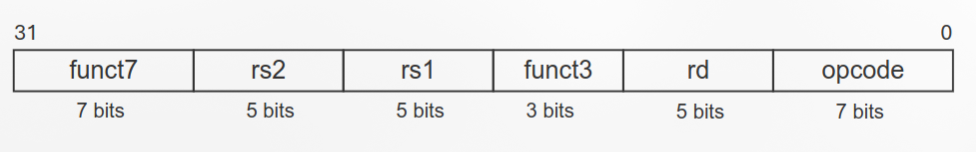
\includegraphics{images/rtype.png}
    \caption{R-type Instructions}
    \label{fig:rtype}
\end{figure}
\begin{itemize}
    \item \texttt{opcode}: partially specifies instruction
    \item \texttt{funct7 + funct3}: combined with opcode, specifies what operation
    \item \texttt{rs1}: first operand (source register 1)
    \item \texttt{rs2}: second operand (source register 2)
    \item \texttt{rd}: destination register (receives the result of the computation)
\end{itemize}
For example, the operation \texttt{x9, x20, x21}
is \texttt{0x015A04B3}.

I-type instructions are immediate arithmetic
and load instructions, and have the form given
in Figure \ref{fig:itype}.
\begin{figure}
    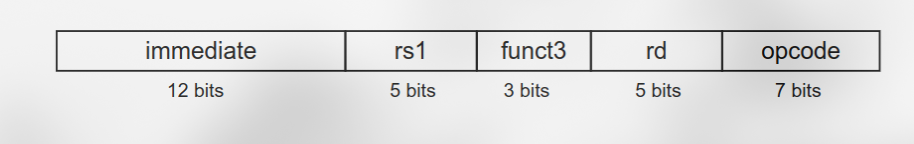
\includegraphics{images/itype.png}
    \caption{I-type Instructions}
    \label{fig:itype}
\end{figure}
\begin{itemize}
    \item \texttt{rs1}: source or base address register number.
    \item \texttt{immediate}: constant operand, or offset added to base address.
\end{itemize}

S-type instructions have the form in
Figure \ref{fig:stype}
\begin{figure}
    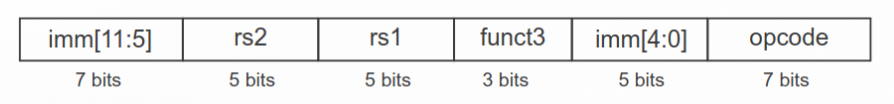
\includegraphics{images/stype.png}
    \caption{S-type Instructions}
    \label{fig:stype}
\end{figure}
\begin{itemize}
    \item \texttt{rs1}: base address register number
    \item \texttt{rs2}: source operand register number
    \item \texttt{immediate}: offset added to base address
\end{itemize}

What separates a computer from a calculator is its ability
to take different actions based on a comparison, e.g. \texttt{if ... else}.

In RISC-V, two conditional branch instructions are
\begin{itemize}
    \item \texttt{beq}: compare two values and branch if equal. What
          happens behind the scenes is that the instruction
          reads the values in the registers and if they are
          equal, jumps program to label
    \item \texttt{bne}: compare and branch if not equal.
\end{itemize}
In both cases, if the comparison is not
true, the program goes to the next instruction.

\begin{lstlisting}[language=C, caption={Conditional Example}]
    // The below assembly is 
    // equivalent to the snippet
    // if (i == j) f = g + h; else f = g - h;
    // in C, if f, g, h, i, j
    // are stored in x19-x23

    bne x22, x23, Else      // go to Else if i != j
    add x19, x20, x12       // f  g + h (skip if i!= j)
    beq x0, x0, Exit        // if 0 == 0, go to Exit
    Else: sub x19, x20, x21 // f = g - h (skip if i == j)
    Exit:
\end{lstlisting}

\begin{lstlisting}[language=C, caption={Loop Example}]
    // The below assembly is 
    // equivalent to the snippet
    // while (save[i] == k)
    //   i += 1;
    // in C

    // a0 = i
    // a1 = k
    // s1 = base address of 'save'

    // Basic block 1
    loop: slli t0, a0, 2 // tmp reg t0 = i * 4
          add t0, t0, s1 // t0 = address save[i]
          lw t2, 0(t0)   // tmp reg t2 = save[i]
    // Basic block 2
          bne t2, a1, exit
          addi a0, a0, 1
    // Basic block 3
          beq x0, x0, loop
    exit:
\end{lstlisting}

A \emph{basic block} is a sequence of
code without a branch or a target,
except at the beginning or end.

Testing for equality is simple and
intuitive. We want to test other
stuff too, like greater than, less than,
greater than or equal to, or
less than or equal to. In RISC-V,
the available instructions are
\begin{itemize}
    \item \texttt{beq}: branch equal
    \item \texttt{bge}: branch greater than or equal
    \item \texttt{bgeu}: unsigned of the above
    \item \texttt{blt}: branch less than
    \item \texttt{bgtu}: unsigned of the above
    \item \texttt{bne}: branch not equal
\end{itemize}
The remaining cases can be constructed
from the provided instructions.

\subsection{Procedures}
Programs more complicated than simple arithmetic need
support for higher-level programming structures. A
universal concept in programming is \emph{procedures},
aka routines, methods, or function calls.

To implement a function call in assembly, we need to be
able to pass arguments, jump to the function, return from
the function, put the result somewhere the caller can see
it, and least obviously, split/fill registers.

Every ISA has a convention for passing parameters to a
function. Typically, the first $N$ arguments are stored
in registers. In RISC-V \texttt{x10}-\texttt{x17}
(alias \texttt{a0}-\texttt{a7}) hold the first 8
function arguments. That means, before you call any
function, the code that calls the function puts the
function arguments in the right order in the registers
\texttt{x10}-\texttt{x17}.

To get to a function, we need to branch to a labelled address.
To get back, we need to remember where we came from. Almost
all ISAs have a special jump-and-link (\texttt{jal}) instruction
which unconditionally moves to the label and stores the location
after the jump in a register.

For a complete example of what's needed in RISC-V to call a function,
see Listing \ref{lst:regargs}.
\begin{lstlisting}[caption={Arguments in Registers}, label={lst:regargs}]
    li x10, 5 // 5 is the first argument
    li a1, 7  // 7 is the second argument (a1 is aliased to x11)
    // Call foo, put the return address in x1
    jal x1, foo

    foo:
        add a0, a0, a1
        // Return to the caller
        jalr x0, 0(x1)
\end{lstlisting}

The temporary registers \texttt{x5}-\texttt{x7} and \texttt{x28}-\texttt{x31},
aliased as \texttt{t0}-\texttt{t6} don't have to be preserved by the called
function. However, the saved registers \texttt{x8}-\texttt{x9}, aliased as
\texttt{s0}-\texttt{s11}, must be preserved by the callee.

A non-leaf function is one that calls other functions. Before it calls
another function, it must preserve its return address and the arguments
and temporaries needed after the call on the stack. When the called function
returns, the calling function must restore the values it had saved to the stack.

\subsection{Stack}

Curious readers may wonder what happens when a function requires more
than 8 parameters, or, in general, what happens when a program needs
more registers to store data than are available. All computers have a
stack data structure to handle copying register value from register to
memory (spills) and getting the register value back from memory to register
(fills). The stack pointer register \texttt{sp} points to the memory address
of the most recently allocated entry of the stack. Pushing moves the stack
pointer to allocate space, then puts register data on the stack. Popping
takes data off the stack, puts it in a register, then moves the stack
pointer to deallocate space.

The stack historically grows down in memory. The stack pointer may start
at some high address like \texttt{0xffff} and be decreased to put new entries
on (spilling). Once those entries are moved back into registers (filling), the stack
pointer increases again. The stack pointer always points to the top of the
stack.

\subsection{Program Counter}
The program counter is a fundamental concept. Every computer has
one. The program counter stores the address of the current instruction in
the special register \texttt{pc}.

Another special register, \texttt{ra}, holds the return address for
after a function call completes. When a function is called, the address
immediately after the current line is pushed into \texttt{ra}. Once the
function call completes (when the \texttt{jalr} instruction is reached),
the program counter is set to the value in \texttt{ra} and the program
resumes execution where it left off. The next time a function call is reached,
the value in \texttt{ra} is changed to the address of the line right
after that function call, and so on.

Functions may have local data that also goes on the stack, such as a local array.
It's useful to know where the frame for each function's data begins.
Some computers will use the register \texttt{fp} to store this frame pointer.

\subsection{Memory Layout}

The memory in a running program is divided into several regions, each
serving a specific purpose. The figure below illustrates a typical layout
in RISC-V systems. The \emph{stack} grows downward from high memory addresses,
while the \emph{heap} grows upward from low addresses. Between them lies a large
unused region reserved for future allocations. The \texttt{.text} section
contains the compiled program instructions, and the \texttt{.data} section
contains global or static variables.

\begin{center}
    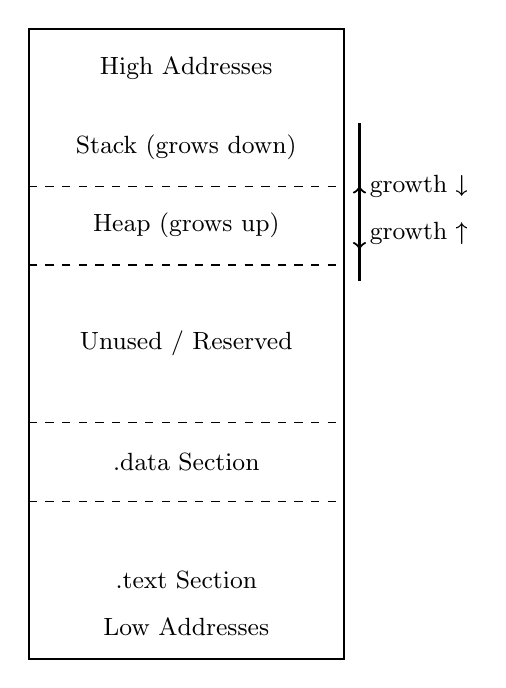
\begin{tikzpicture}[font=\small]
        % Memory column
        \draw[thick] (0,0) rectangle (4,8);
        \draw[dashed] (0,6) -- (4,6);
        \draw[dashed] (0,5) -- (4,5);
        \draw[dashed] (0,3) -- (4,3);
        \draw[dashed] (0,2) -- (4,2);

        % Labels
        \node at (2,7.5) {High Addresses};
        \node at (2,6.5) {Stack (grows down)};
        \node at (2,5.5) {Heap (grows up)};
        \node at (2,4) {Unused / Reserved};
        \node at (2,2.5) {.data Section};
        \node at (2,1) {.text Section};
        \node at (2,0.4) {Low Addresses};

        % Arrows showing growth
        \draw[->, thick] (4.2,6.8) -- (4.2,5.2) node[midway, right]{growth ↓};
        \draw[->, thick] (4.2,4.8) -- (4.2,6.0) node[midway, right]{growth ↑};
    \end{tikzpicture}
\end{center}

\paragraph{The \texttt{.text} Section}
The \texttt{.text} section of a program holds the compiled machine instructions
that make up the executable code. This region is typically marked as
read-only to prevent accidental modification of instructions at runtime.

\paragraph{The \texttt{.data} Section}
The \texttt{.data} section stores global and static variables that have been
initialized before the program starts running. Variables declared with
initial values (like \texttt{int x = 5;}) reside here, while uninitialized
globals are placed in a separate \texttt{.bss} section.

\subsection{Application Binary Interface}

The Application Binary Interface (ABI) defines how compiled code interacts at
the binary level. It specifies calling conventions, register usage, stack
organization, and how data types are represented in memory. The ABI ensures
that separately compiled modules, such as libraries and user code, can
work together correctly. In RISC-V, the ABI defines which registers
hold function arguments and return values, which must be preserved across
calls, and how the stack frame is structured.

\begin{table}[h]
    \centering
    \caption{Register Conventions}
    \begin{tabular}{|c|c|l|c|}
        \hline
        \textbf{Name} & \textbf{Register Number} & \textbf{Usage}                 & \textbf{Preserved on Call?} \\
        \hline
        x0            & 0                        & The constant value 0           & n.a.                        \\
        x1 (ra)       & 1                        & Return address (link register) & yes                         \\
        x2 (sp)       & 2                        & Stack pointer                  & yes                         \\
        x3 (gp)       & 3                        & Global pointer                 & yes                         \\
        x4 (tp)       & 4                        & Thread pointer                 & yes                         \\
        x5-x7         & 5-7                      & Temporaries                    & no                          \\
        x8-x9         & 8-9                      & Saved                          & yes                         \\
        x10-x17       & 10-17                    & Arguments/results              & no                          \\
        x18-x27       & 18-27                    & Saved                          & yes                         \\
        x28-x31       & 28-31                    & Temporaries                    & no                          \\
        \hline
    \end{tabular}
\end{table}
